%**********************************************************
%\subsection{Task Overview}
One can define and describe briefly how the local system is implemented, making use of threads and processes. As one can see in figure \ref{fig:task_overview}, this system is composed by two processes: the main process and a daemon, \textit{dSensors}, used to read the sensors \textit{LDR}, \textit{PIR} and \textit{LampFailureDetector}. The communication between the daemon and the main process is done via message queue and through the use of the signal \textit{SIGUSR1}, which the daemon can use to notify the main process of when there is a new message to read in the message queue.

\begin{figure}[H]
	\centering
	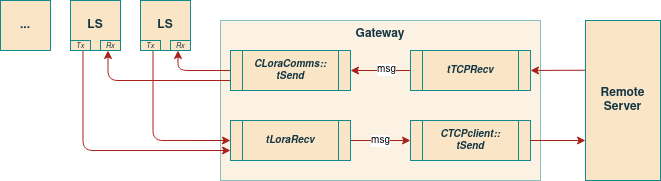
\includegraphics[width=.4\textwidth]{09sw_specification/LS/overview}
	\caption{Inter-process Communication between Main Process and Daemon.}
	\label{fig:task_overview}
\end{figure}

%**********************************************************
\subsection{Class Diagrams}
In figure \ref{fig:clocalsystem} is represented the class diagram of the local system's main process. The class \textit{CLocalSystem} is the main class of the main process, which initializes the objects of each class listed below.

\begin{itemize}
	\item \textbf{CLoraComm:} manages the LoRa communications with the gateway, interfacing with the LoRa module;
	\item \textbf{CLamp:} manages the lamp brightness, using a PWM signal;	
	\item \textbf{CCamera:} manages the camera device;
	\item \textbf{CParkDetection:} responsible of image processing for detecting parking spots.
\end{itemize}

\begin{figure}[H]
	\centering
	\includegraphics[width=1\textwidth]{09sw_specification/LS/clocalsystem/class}
	\caption{Local System Main Process Class Diagram.}
	\label{fig:clocalsystem}
\end{figure}

\clearpage
In figure \ref{fig:csensors} is represented the class diagram of the local system's daemon. The class \textit{CSensors} is the main class of dSensors, which initializes all objects of each class listed bellow.

\begin{itemize}
	\item \textbf{CPir:} manages the motion detector, PIR;
	\item \textbf{CLdr:} manages the ambient light sensor, LDR;
	\item \textbf{CFailureDetector:} manages the lamp failure detector;
\end{itemize}

\begin{figure}[H]
	\centering
	\includegraphics[width=0.7\textwidth]{09sw_specification/LS/csensors/class}
	\caption{Local System dSensors Class Diagram.}
	\label{fig:csensors}
\end{figure}

%*****************************
\clearpage
\myparagraph{Class CLoraComm}

In figure \ref{fig:LoraCommClass} is shown the \textit{CLoraComm} class diagram. This class defines an object \textit{CLoraComm}, with the address \textit{local\_addr}, capable of establishing a LoRa communication at a defined frequency \textit{freqMHz}, with the gateway which has the address \textit{dest\_addr}. This class inherits several methods from the class \textit{CCommunication}, represented with a lighter font and identified with '\^{}' at the begin of the method, which will be specified later.

\begin{figure}[H]
	\centering
	\includegraphics[width=.4\textwidth]{09sw_specification/LS/cloracomm/class}
	\caption{Class Diagram: CLoraComm.}
	\label{fig:LoraCommClass}
\end{figure}

%*****************************
\clearpage
\myparagraph{Class CCommunication}

In figure \ref{fig:CCommunicationClass} is shown the \textit{CCommunication} class diagram. This class implements the structure for a communication class like \textit{CLoraComm} or \textit{CTCPclient}, which will be shown later. It implements a series of methods to send and receive messages. 

This class makes use of a thread, \textit{tSend}, to send messages in non-blocking mode. This thread is created with \textit{init(tprio)} method, which defines the thread priority and creates it. After creation, the thread goes to sleep, and is waken whenever the condition variable \textit{condtSend} is notified, which occurs when \textit{push(msg)} is used. This function adds the given message to a buffer, \textit{TxMsgs}, which is later sent in \textit{tSend}. This way, one has a waiting list of messages to be sent, in order to avoid the loss of a communication. The method \textit{send(msg)} sends a message in blocking mode; \textit{recv()} receives a message in non-blocking mode.

This class has two pure virtual functions: \textit{recvFunc} and \textit{sendFunc}, which must be implemented by the derived classes, since each communication protocol has its own functions to send and receive messages. Each communication has a state, \textit{status}, defined by the enumeration connection status, \textit{ConnStatus}.

\begin{figure}[H]
	\centering
	\includegraphics[width=.68\textwidth]{09sw_specification/LS/ccommunication/class}
	\caption{Class Diagram: CCommunication.}
	\label{fig:CCommunicationClass}
\end{figure}

%*****************************
\clearpage
\myparagraph{Class CLamp}

In figure \ref{fig:classlamp} is shown the \textit{CLamp} class diagram, which defines a \textit{CLamp} object. When creating the object, using the constructor \textit{CLamp()}, one can define how much time the lamp stays at maximum brightness, passing this time to the constructor through parameter, \textit{timeoutSecs}, in seconds, being defined into \textit{LampOnTimeoutSecs}.
One can interact with the object \textit{CLamp} by changing the brightness, through the method \textit{setBrightness(lux)}, where \textit{lux} is a value from 0, where the lamp is OFF, to 100, where the lamp is at maximum brightness.  Internally, this class uses a mutex, \textit{mutChangePWM} to protect the PWM value when using \textit{setBrightness} method. 

\begin{figure}[H]
	\centering
	\includegraphics[width=.4\textwidth]{09sw_specification/LS/clamp/class}
	\caption{Class Diagram: CLamp.}
	\label{fig:classlamp}
\end{figure}

%*****************************
%\clearpage
\myparagraph{Class CPir}

In figure \ref{fig:classpir} is shown the \textit{CPir} class. When movement is detected in the surrounding area of the lamppost, the sensor puts the high digital value in its output, triggering an interrupt service routine. When creating a object \textit{CPir}, one can define the ISR to be executed, passing to the constructor a function pointer, \textit{pirISR}.

\begin{figure}[H]
	\centering
	\includegraphics[width=.4\textwidth]{09sw_specification/LS/cpir/class}
	\caption{Class Diagram: CPir.}
	\label{fig:classpir}
\end{figure}

%*****************************
\myparagraph{Class CCamera}

In figure \ref{fig:classcamera} is shown the \textit{CCamera} class diagram, that defines a camera object.  This class implements the control of a camera device, with filename \textit{camFilename}, through the basic functions \textit{open()}, \textit{close()} and \textit{capture()}, the latter used to get an image frame from the camera.

\begin{figure}[H]
	\centering
	\includegraphics[width=.4\textwidth]{09sw_specification/LS/ccamera/class}
	\caption{Class Diagram: CCamera.}
	\label{fig:classcamera}
\end{figure}

%*****************************
\clearpage
\myparagraph{Class CParkDetection}

In figure \ref{fig:classcamera} is shown the \textit{CParkDetection} class diagram, that implements the tools needed to do process camera frames in order to do parking detection. Before determining if there are parking spots available, one needs to extract the park outline from the camera frame, using \textit{getOutline(frame)}. This method stores in the variable \textit{parkCoords} the coordinates on the image frame relating to the park outline. After this, one can calculate the number of vacants inside that park outline, through \textit{calcVacants(frame)}.

\begin{figure}[H]
	\centering
	\includegraphics[width=.34\textwidth]{09sw_specification/LS/cparkdetection/class}
	\caption{Class Diagram: CParkDetection.}
	\label{fig:classparkdetection}
\end{figure}

%*****************************
\clearpage
\myparagraph{Class CLdr}

In figure \ref{fig:classldr} is shown the \textit{CLdr} class, that defines the functions to interact with the LDR sensor. This contains an enumeration for the luminosity states, \textit{LuxState}, which can be \textit{DAY}, \textit{NIGHT} or \textit{UNDEF} as undefined, used for initialization. The luminosity state can be obtain by the use of \textit{getLuxState()}. This class also contains a structure \textit{LdrTxFrame}, which relates each \textit{LuxState} to a command, that will be sent to the main process, whenever \textit{LuxState} changes. Using \textit{getStateCmd()} one can get the command associated with the current \textit{luxState}. The command list, \textit{cmdList}, is defined in the constructor with the following commands:
\begin{itemize}
	\item "OFF" for when the LuxState is "DAY". When the LDR detects that is day time, the \textit{luxState} changes to \textit{DAY}, and at that moment is sent the command \textit{"OFF"} to the main process, in order to turn off the lamp;
	\item "MIN" for when the LuxState is "NIGHT". When the LDR detects that is night time, the \textit{lusState} changes to \textit{NIGHT}, and at that moment is sent the command \textit{"MIN"}, in order to put the lamp at minimum brightness.
\end{itemize}

%that defines the functions to interact with the LDR sensor, using its device driver. As the ambient light is read each 10 minutes in the function \textit{LdrIsr}, one needs to define a timer to trigger this function. The last read luminance is stored in the variable \textit{oldLightCon} and is obtained using the function \textit{getLux}.
\begin{figure}[H]
	\centering
	\includegraphics[width=0.74\textwidth]{09sw_specification/LS/cldr/class}
	\caption{Class Diagram: CLdr.}
	\label{fig:classldr}
\end{figure}

%*****************************
\clearpage
\myparagraph{Class CFailureDetector}

In figure \ref{fig:classfail} is shown the Failure Detector class. After creating an instance of this class, using the contructor \textit{FailureDetector}, the function \textit{failureDetectIsr} will be triggered each time the failure detector senses the lamp failure. 

\begin{figure}[H]
	\centering
%	\includegraphics[width=.5\textwidth]{09sw_specification/LS/cfail}
	\caption{Class Diagram: CFailureDetector.}
	\label{fig:classfail}
\end{figure}

%**********************************************************
\clearpage
\subsection{Task Overview}

One can list the tasks that compose the main process:
\begin{itemize}
 	\item \textbf{CLoraComm::tSend:} sends a message to the gateway, using the LoRa module;
	\item \textbf{CLocalSystem::tParkDetection:} determines parking outline; acquire a camera frame, process it by verifying parking spots availability;
	\item \textbf{CLocalSystem::tLoraRecv:} receives a message from the gateway, using the LoRa module;
	\item \textbf{CLocalSystem::tRecvSensor:} receives messages sent by the daemon, via message queue, regarding sensors information. It's awaken by the use of signal \textit{SIGUSR1}, sent by the daemon when there is a message to read.
\end{itemize}

Bellow are listed the tasks that compose the daemon, \textit{dSensors}. As stated above, in \textit{tRecvSensor}, whenever one of the following tasks sends a command to the main process, it is done by message queue, and also, a signal is used, \textit{SIGUSR1}, to alert the main process that a new message was sent.
\begin{itemize}
	\item \textbf{CSensors::tReadLdr:} periodically reads the LDR sensor; if a change in luminosity state is detected (\textit{DAY} to \textit{NIGHT}, or vice-versa) a command is sent to the main process;
	\item \textbf{CSensors::tReadLampf:} periodically reads the Lamp Failure Detector; if a failure is detected a command is sent to the main process;
	\item \textbf{CSensors::PirISR:} ISR for the PIR sensor; when motion is detected this task is executed and a command is sent to the main process. 
\end{itemize}

%**********************************************************
\clearpage
\subsection{Task Priority}

One needs to assign each thread a static priority level to indicate their relative urgency. Moreover, the scheduler will always pick the thread that is ready to execute with the highest priority level. Priorities must be assigned in order to ensure efficiency and execute real-time tasks.

With that in mind, the priority assignment diagram for the local system's main process is represented in figure \ref{fig:lst_priority}, as well as for the daemon, in figure \ref{fig:lsdaemont_priority}.

\begin{figure}[H]
	\centering
	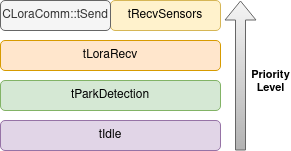
\includegraphics[width=.6\textwidth]{09sw_specification/LS/mainprocess_priority}
	\caption{Local System Main Process Priority Assignment Schematic.}
	\label{fig:lst_priority}
\end{figure}

\begin{figure}[H]
	\centering
	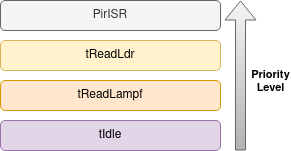
\includegraphics[width=.6\textwidth]{09sw_specification/LS/dsensors_priority}
	\caption{Local System dSensors Priority Assignment Schematic.}
	\label{fig:lsdaemont_priority}
\end{figure}

%**********************************************************
\clearpage
\subsection{Task Synchronization}
Real-time tasks share resources and services, and as such, should be prepared to await for the availability of these resources and services, like logical resources (buffers and data), physical resources, services like directory services, etc. In order to have coordinate access to shared resources and avoid race conditions, the kernel has resources that provide synchronization tools. 

\myparagraph{Condition Variables}

A condition variable is a task synchronization tool that can be used to block (wait) one or more threads, suspending its execution. The blocked threads are awakened when the condition variable is notified. 

The condition variables used in the main process are listed below.

\begin{itemize}
	\item \textbf{CLocalSystem::condRecvSensors:} notifies \textit{tRecvSensors} that a new message is available on the message queue, \textit{msgqSensors};

	\item \textbf{CLocalSystem::condCamFrame:} notifies \textit{tParkDetection} to acquire a new camera frame and process it;

	\item \textbf{CCommunication::condtSend:} used to notify \textit{CCommunication::tSend} that a new message is ready to be sent.
\end{itemize}

The condition variables used in the daemon are listed below.

\begin{itemize}
	\item \textbf{CSensors::condReadLdr:} notifies \textit{tReadLdr} to acquire values from LDR sensor and process them;

	\item \textbf{CSensors::condReadLampf:} notifies \textit{tReadLampf} to acquire values from Lamp Failure Detector and process them;
\end{itemize}

\myparagraph{Mutexes}

A mutex is a locking mechanism that provides mutual exclusion, supporting ownership and other protocols. A mutex is initially created in the unlocked state in which it can be acquired by a task. After being acquired, the mutex moves to the locked state. When the task releases the mutex, it returns to the unlocked state.

\clearpage
The mutexes used in the main process are listed bellow.

\begin{itemize}
	\item \textbf{CLocalSystem::mutRecvSensors:} mutex associated with the condition variable \textit{condRecvSensors} to read a new message from the sensors message queue;

	\item \textbf{CLocalSystem::mutCamFrame:} mutex associated with the condition variable \textit{condCamFrame} to acquire a camera frame;

	\item \textbf{CCommunication::mutComms:} indirectly used by \textit{CLoraComms}, to protect communication usage of send and receive functions;

	\item \textbf{CCommunication::mutTxMsgs:} indirectly used by \textit{CLoraComms}; used to protect the insertion and removal of messages into \textit{TxMsgs};

	\item \textbf{CLamp::mutChangePWM:} protects the modification of PWM when defining a new PWM value for the lamp.
\end{itemize}

The mutexes used in the daemon are listed bellow.

\begin{itemize}
	\item \textbf{CSensors::mutReadLdr:} protects reading of LDR sensor;
	\item \textbf{CSensors::mutReadLampf:} protects reading of Lamp Failure Detector.
\end{itemize}

\myparagraph{Signals}

A signal is a notification to a process that an event has occurred. Signals are sometimes described as software interrupts, being analogous to hardware interrupts in that they interrupt the normal flow of execution of a program. One process can send a signal to another process, being in that way, employed as a synchronization technique.

The signals used between the main process and the daemon are listed bellow.

\begin{itemize}
	\item \textbf{SIGUSR1:}	signal sent by \textit{dSensors} to the main process, whenever a new message is inserted in the message queue, \textit{msgqSensors}. This is received in the main process in a signal handler, that will wake up the task \textit{tRecvSensors}, through the condition variable \textit{condRecvSensors}.
\end{itemize}

%**********************************************************
\subsection{Task Communication}
\myparagraph{Message Queue}

A message queue is a linked list of messages stored within the kernel and identified by a message queue identifier. A message queue, \textit{msgqSensors}, will be used to communicate between the main process and the \textit{dSensors}. In that way, the main process is agnostic to the cyclic reading necessary for the sensors \textit{LDR} and \textit{LampFailureDetector}, and is only informed when necessary, through the message queue.

%**********************************************************
\subsection{Start-Up Process}

\myparagraph{Main Process}

The start-up for the main process is shown in figure \ref{fig:mainprocess}. Firstly, a \textit{CLocalSystem} object is created, initializing all objects, that will be detailed later. After that, \textit{run()} method from \textit{CLocalSystem} is used, which will wait for the termination of all tasks.

\begin{figure}[H]
	\centering
	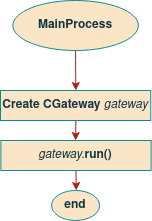
\includegraphics[width=.3\textwidth]{09sw_specification/LS/mainprocess}
	\caption{Start-Up Process: Main Process.}
	\label{fig:mainprocess}
\end{figure}

\clearpage
\myparagraph{dSensors}

The start-up for the daemon is shown in figure \ref{fig:dsensors}. Firstly, the process becomes a daemon, being that represented by \textit{daemonize()}. After that, a message queue is opened in order to communicate with the main process. Then, it will wait until it receives a message in the message queue, that will be the main process PID. After this setups, a \textit{CSensors} object is created, and the \textit{run()} method is used, working similarly to the one presented in the main process start-up process.

\begin{figure}[H]
	\centering
	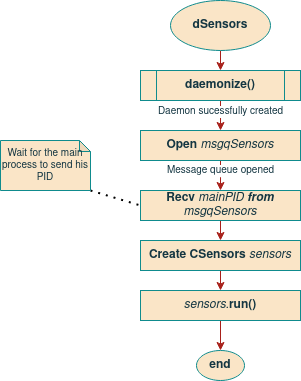
\includegraphics[width=.55\textwidth]{09sw_specification/LS/dsensors}
	\caption{Start-Up Process: dSensors.}
	\label{fig:dsensors}
\end{figure}

%**********************************************************
\clearpage
\subsection{Flowcharts}
%**********************************************************
\myparagraph{CLocalSystem Methods}

The class constructor is shown in figure \ref{fig:CLocalSystemConstructor}. This is responsible for initializing all synchronization tools and private variables used, as well as creating the tasks \textit{tLoraRecv}, \textit{tRecvSensors} and \textit{tParkDetection}.

\begin{figure}[H]
	\centering
	\includegraphics[width=.3\textwidth]{09sw_specification/LS/clocalsystem/constructor}
	\caption{Flowchart: CLocalSystem constructor.}
	\label{fig:CLocalSystemConstructor}
\end{figure}

%******************************
\clearpage
The method \textit{run()}, presented in figure \ref{fig:CLocalSystemRun}, it's implemented similarly in various classes. This is responsible for starting timers that trigger the execution of tasks, and wait (\textit{join}) for the termination of the tasks.

\begin{figure}[H]
	\centering
	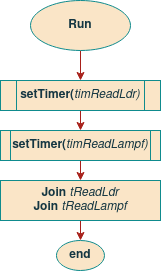
\includegraphics[width=.3\textwidth]{09sw_specification/LS/clocalsystem/run}
	\caption{Flowchart: CLocalSystem Run method.}
	\label{fig:CLocalSystemRun}
\end{figure}

%******************************
\clearpage
In figure \ref{fig:CLocalSystemtLoraRecv} is presented the task responsible for receiving a message from the gateway, via LoRa communication, parse it and execute the respective command.

\begin{figure}[H]
	\centering
	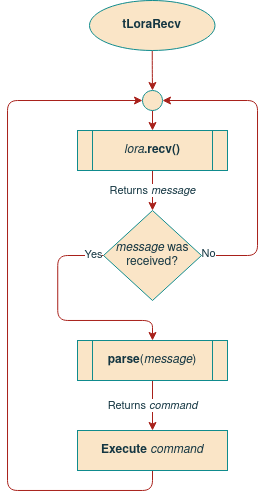
\includegraphics[width=.54\textwidth]{09sw_specification/LS/clocalsystem/tlorarecv}
	\caption{Flowchart: CLocalSystem tLoraRecv method.}
	\label{fig:CLocalSystemtLoraRecv}
\end{figure}

%******************************
\clearpage
In figure \ref{fig:CLocalSystemtRecvSensors} is presented the task responsible for receiving messages from the sensors daemon, via message queue. When there are no messages to read from the message queue, the task goes to sleep and is awaken when \textit{condRecvSensors} is notified. This happens in the \textit{sigHandler}, presented in figure \ref{fig:CLocalSystemsigHandler}, which is the signal handler for the main process, being this in charge of signaling the condition variable \textit{condRecvSensors} when a \textit{SIGUSR1} signal is catched.

\begin{figure}[H]
	\centering
	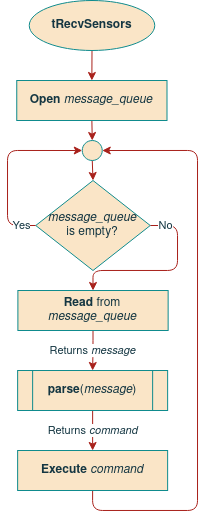
\includegraphics[width=1\textwidth]{09sw_specification/LS/clocalsystem/trecvsensors}
	\caption{Flowchart: CLocalSystem tRecvSensors method.}
	\label{fig:CLocalSystemtRecvSensors}
\end{figure}

\begin{figure}[H]
	\centering
	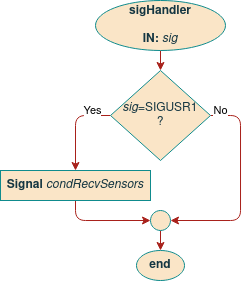
\includegraphics[width=.5\textwidth]{09sw_specification/LS/clocalsystem/sighandler}
	\caption{Flowchart: CLocalSystem sigHandler method.}
	\label{fig:CLocalSystemsigHandler}
\end{figure}

%******************************
\clearpage
This task, figure \ref{fig:CLocalSystemtParkDetection}, is responsible for using the \textit{camera} object, from \textit{CCamera}, and the \textit{park} object, from \textit{CParkDetection}, in order to capture image frames and process them, calculating the number of available spaces in the parking detected. This task is periodically awaken by the use of a timer, signaling the condition variable \textit{condCamFrame}. Besides that, a timer can be used, \textit{timCamProc}, to detect if the image processing does not exceed a maximum amount of time.

\begin{figure}[H]
	\centering
	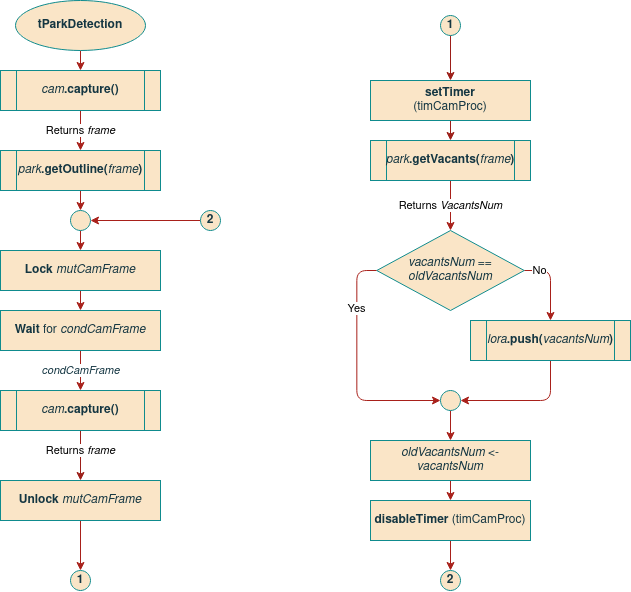
\includegraphics[width=1\textwidth]{09sw_specification/LS/clocalsystem/tparkdetection}
	\caption{Flowchart: CLocalSystem tParkDetection method.}
	\label{fig:CLocalSystemtParkDetection}
\end{figure}

%**********************************************************
\clearpage
\myparagraph{CSensors Methods}

As in the previous class, the class constructor and the \textit{run()} method serves similar purposes, therefore, one has no need to specify them.\\

In figure \ref{fig:CSensorstreadldr} is shown the task responsible for reading luminosity values using the LDR sensor. If there is a change in the luminosity state, to the state NIGHT, this task enables the lamp failure detector, \textit{lampf}, and the motion detector, \textit{pir}, and then, a command is sent to the main process, using \textit{sendCmd(cmd)} method, indicating that the lamp should be turned on at minimum bright. If the change in the luminosity state is to the state DAY, the opposite occurs, disabling the detectors, and sending a command to the main process, indicating that the lamp should be off.

\begin{figure}[H]
	\centering
	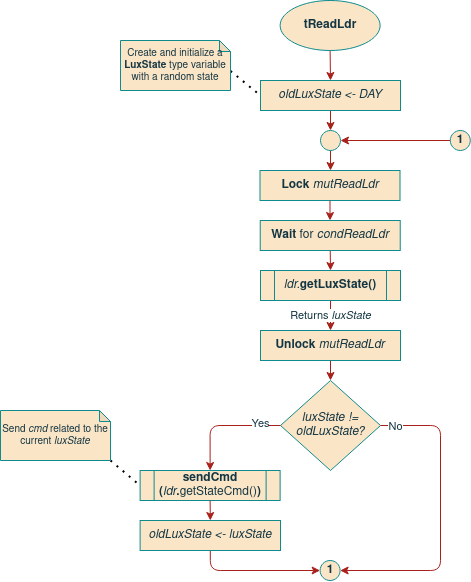
\includegraphics[width=1\textwidth]{09sw_specification/LS/csensors/treadldr}
	\caption{Flowchart: CSensors tReadLdr method.}
	\label{fig:CSensorstreadldr}
\end{figure}

%******************************
\clearpage
The method \textit{PirISR}, is executed when there is motion detected, sending the \textit{"ON"} command to the main process, indicating that the lamp should be at maximum bright.

\begin{figure}[H]
	\centering
	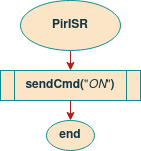
\includegraphics[width=.3\textwidth]{09sw_specification/LS/csensors/pirisr}
	\caption{Flowchart: CSensors PirISR method.}
	\label{fig:CSensorspirisr}
\end{figure}

%******************************
The method \textit{lampfISR} is very similar to the \textit{PirISR}, since it is executed when the lamp failure detector detects that the lamp is off, when it shouldn't. This sends a command to the main process, \textit{"FAIL"}, indicating that there was detected a failure in the lamp and that it should be turned off.

\begin{figure}[H]
	\centering
	\includegraphics[width=.3\textwidth]{09sw_specification/LS/csensors/lampfISR}
	\caption{Flowchart: CSensors lampfISR method.}
	\label{fig:CSensorstreadlampf}
\end{figure}

%******************************
\clearpage
The method \textit{sendCmd}, shown in figure \ref{fig:CSensorssendcmd}, is responsible for sending a string, \textit{cmd}, to the message queue, \textit{msgqSensors}. After that, it sends a signal, \textit{SIGUSR1}, to the process \textit{mainPID}, which is the main process PID.

\begin{figure}[H]
	\centering
	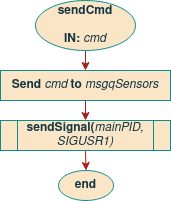
\includegraphics[width=.35\textwidth]{09sw_specification/LS/csensors/sendcmd}
	\caption{Flowchart: CSensors sendCmd method.}
	\label{fig:CSensorssendcmd}
\end{figure}

%**********************************************************
\clearpage
\myparagraph{CCommunication Methods}

The class constructor is shown in figure \ref{fig:CCommunicationConstructor}. This is responsible for initializing all synchronization tools and private variables used.

\begin{figure}[H]
	\centering
	\includegraphics[width=.3\textwidth]{09sw_specification/LS/ccommunication/constructor}
	\caption{Flowchart: CCommunication constructor.}
	\label{fig:CCommunicationConstructor}
\end{figure}

%******************************
To send a message, this class has a built-in thread, \textit{tSend} that can be created using \textit{init(tprio)}, which expects a priority for the thread, \textit{tprio}, as shown in figure \ref{fig:CCommunicationinit}.

\begin{figure}[H]
	\centering
	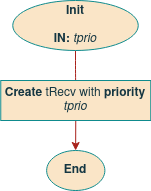
\includegraphics[width=.3\textwidth]{09sw_specification/LS/ccommunication/init}
	\caption{Flowchart: CCommunication Init method.}
	\label{fig:CCommunicationinit}
\end{figure}

%******************************
A message can be put in the waiting list to be sent through the use of \textit{push(msg)}, as shown in figure \ref{fig:CCommunicationPush}. This function is responsible for adding a new message, \textit{msg}, to the \textit{TxMsgs} vector, and signal the condition variable \textit{condSend}, for the thread \textit{tSend} to send the message.

\begin{figure}[H]
	\centering
	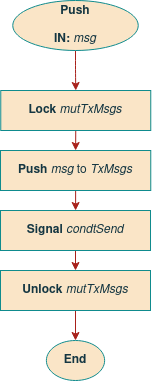
\includegraphics[width=.3\textwidth]{09sw_specification/LS/ccommunication/push}
	\caption{Flowchart: CCommunication Push method.}
	\label{fig:CCommunicationPush}
\end{figure}

%******************************
\clearpage
This thread, \textit{tSend} presented in figure \ref{fig:CCommunicationtsend}, is responsible for sending queued messages to the gateway, using LoRa communication. A conditional variable is used to wake this thread when there is a new message available to be sent. When the queue \textit{TxMsgs} is empty, the task goes to sleep, waiting for the condition variable \textit{condSend} to notify this task. After this, the mutex \textit{mutComms} is used to protect the communication. Then, a message is popped from the messages queue, and sent to the gateway using the method \textit{Send}, shown in figure \ref{fig:CCommunicationsend}. This continues to happen until the \textit{TxMsgs} queue gets empty.

\begin{figure}[H]
	\centering
	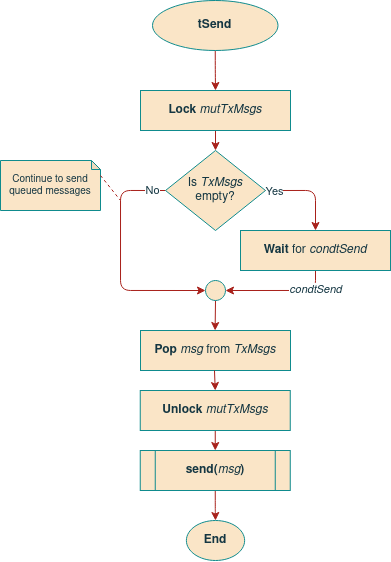
\includegraphics[width=.682\textwidth]{09sw_specification/LS/ccommunication/tsend}
	\caption{Flowchart: CCommunication tSend thread.}
	\label{fig:CCommunicationtsend}
\end{figure}

\begin{figure}[H]
	\centering
	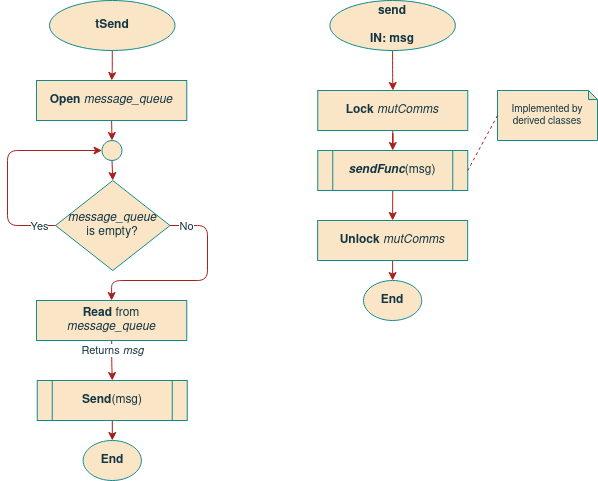
\includegraphics[width=.55\textwidth]{09sw_specification/LS/ccommunication/send}
	\caption{Flowchart: CCommunication Send method.}
	\label{fig:CCommunicationsend}
\end{figure}

%******************************
\clearpage
There is also another method, \textit{recv()}, that receives a message from the gateway, in a non blocking mode, making use of task synchronization tools to ensure that sending and receiving don't occur at the same time. This function should be used continuously if one doesn't want to miss any communication. This method is presented in figure \ref{fig:CCommunicationrecv}.

\begin{figure}[H]
	\centering
	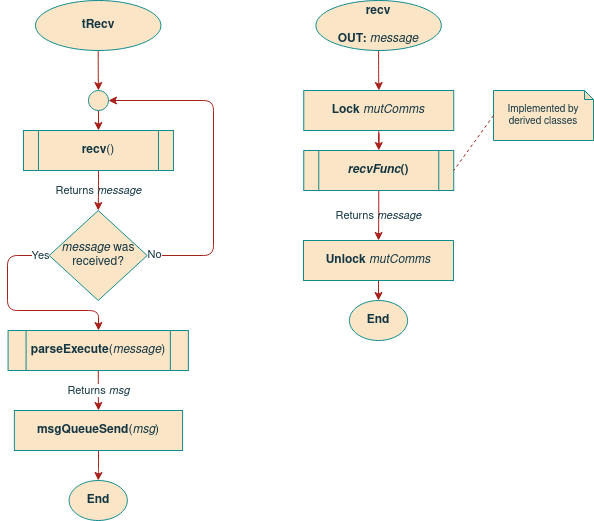
\includegraphics[width=.55\textwidth]{09sw_specification/LS/ccommunication/recv}
	\caption{Flowchart: CCommunication Recv method.}
	\label{fig:CCommunicationrecv}
\end{figure}

%**********************************************************
\clearpage
\myparagraph{CLoraComm Methods}

A CLoraComm object can be created through the use of the constructor, as shown in figure \ref{fig:LoraComm}.
This starts by initializing the LoRa communication, using the given frequency, \textit{freq}, which will be 433~MHz, and defining the pins connected to the module. At the end, all private members are also initialized.

\begin{figure}[H]
	\centering
	\includegraphics[width=.6\textwidth]{09sw_specification/LS/cloracomm/constructor}
	\caption{Flowchart: CLoraComm constructor.}
	\label{fig:LoraComm}
\end{figure}

This class inherits from \textit{CCommunication} class, so this must implement \textit{recvFunc} and \textit{sendFunc}, as they are pure virtual methods. In this class, one will use existent functions \textit{LoraReceive} and \textit{LoraSend} to implement Lora communication, as shown in figures \ref{fig:CLoraCommrecvfunc} and \ref{fig:CLoraCommsendfunc}. This functions make use of the address of the local system, \textit{local\_addr}, defining the source ID, and the address of the gateway, \textit{dest\_addr}, defining the destination ID.

\begin{figure}[H]
	\centering		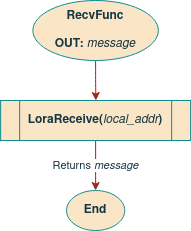
\includegraphics[width=.4\textwidth]{09sw_specification/LS/cloracomm/recvfunc}
	\caption{Flowchart: CLoraComm recvFunc method.}
	\label{fig:CLoraCommrecvfunc}
\end{figure}

\begin{figure}[H]
	\centering
	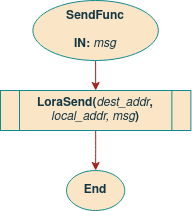
\includegraphics[width=.4\textwidth]{09sw_specification/LS/cloracomm/sendfunc}
	\caption{Flowchart: CLoraComm sendFunc method.}
	\label{fig:CLoraCommsendfunc}
\end{figure}


%**********************************************************
\clearpage
\myparagraph{CLamp Methods}

A CLamp object can be created through the class constructor, presented in figure \ref{fig:CLampconstructor}. When creating an object, one must pass to the constructor the time from which the lamp will stay on after one sets the brightness to the maximum. This value must be in seconds and is stored in the variable \textit{timLampOnSecs}.

\begin{figure}[H]
	\centering	
	\includegraphics[width=.35\textwidth]{09sw_specification/LS/clamp/constructor}
	\caption{Flowchart: CLamp constructor.}
	\label{fig:CLampconstructor}
\end{figure}

%******************************
This functions, presented in figure \ref{fig:CLamponoff}, are responsible for enabling and disabling the PWM for the lamp, which is responsible for controlling the lamp brightness. When turning on the lamp PWM, one can define the lamp brightness level, through \textit{lux} argument.

\begin{figure}[H]
	\centering	
	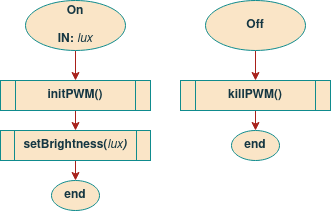
\includegraphics[width=.5\textwidth]{09sw_specification/LS/clamp/onoff}
	\caption{Flowchart: CLamp On and Off methods.}
	\label{fig:CLamponoff}
\end{figure}

%******************************
\clearpage
This function, presented in figure \ref{fig:CLampsetBrightness}, is responsible for changing the PWM associated with the lamp, which is directly related to its brightness. Through \textit{setPWM(lux)} one can change the applied lamp PWM to \textit{lux} value, being this an integer between 0 to 100. When the PWM is maximum, a timer is started that defines how much time the lamp is ON, \textit{timLampOnSecs} in seconds.

\begin{figure}[H]
	\centering	
	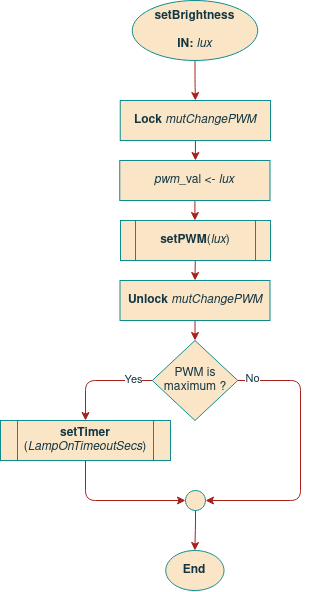
\includegraphics[width=.57\textwidth]{09sw_specification/LS/clamp/setbrightness}
	\caption{Flowchart: CLamp setBrightness method.}
	\label{fig:CLampsetBrightness}
\end{figure}

%**********************************************************
\clearpage
\myparagraph{CParkDetection Methods}

In the method \textit{calcVacantsNum()}, one receives an image frame and processes it in order to determine the number of available parking spots. This does the detection of cars using a pre-trained model. When analyzing the image, if the coordinates of a detected car matches the coordinates of the parking spot (i.e the parking outline, obtained by \textit{getOutline()}) then one can assume that the parking spot is occupied. \\

%******************************
This method, represented in figure \ref{fig:CParkDetectiongetoutline}, is used to process the image captured by the camera in order to detect the parking spots outline. This is done using the algorithm defined previously in the section \ref{section:imageProc}, and starts by converting the frame to a grey scale image, apply the canny edge filter to highlight the edges of the image captured. After having the edges, one can select only the vertical and horizontal straight lines and intersect them, storing the intersection points, that are the parking spot coordinates, into the private member \textit{parkCoords}.

\begin{figure}[H]
	\centering			
	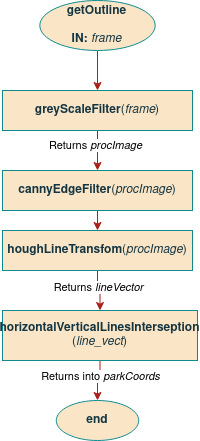
\includegraphics[width=.4\textwidth]{09sw_specification/LS/cparkdetection/getoutline}
	\caption{Flowchart: CParkDetection getOutline method.}
	\label{fig:CParkDetectiongetoutline}
\end{figure}

%**********************************************************
\clearpage
\myparagraph{CLdr Methods}

The constructor for the class \textit{CLdr} is presented in \ref{fig:CLdrconstructor}. This creates an \textit{CLdr} object, initializing the LDR sensor, defining the initial luminosity state, \textit{luxState}.

\begin{figure}[H]
	\centering
	\includegraphics[width=.3\textwidth]{09sw_specification/LS/cldr/constructor}
	\caption{Flowchart: CLdr constructor.}
	\label{fig:CLdrconstructor}
\end{figure}

%******************************
\clearpage
In order to obtain the current luminosity state, \textit{DAY} or \textit{NIGHT}, there is a method called \textit{getLuxState}, presented in figure \ref{fig:CLdrgetLuxState}. This method, gets the sensed luminosity level from the LDR sensor, and determines the current luminosity state.

\begin{figure}[H]
	\centering
	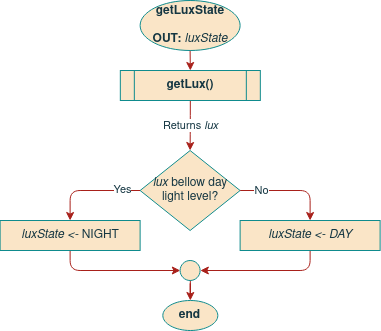
\includegraphics[width=.75\textwidth]{09sw_specification/LS/cldr/getluxstate}
	\caption{Flowchart: CLdr getLuxState method.}
	\label{fig:CLdrgetLuxState}
\end{figure}

%**********************************************************
\clearpage
\myparagraph{CPir Methods}

In figure \ref{fig:CPirconstructor} is shown the CPir class constructor. This creates a CPir object, by firstly inserting the respective device driver, which will be developed, as a constraint of this project. Then an ISR is assigned to the PIR sensor, being that defined by a function pointer passed by argument into the constructor. Whenever the PIR detects movement in the surroundings, the output pin will change its value, triggering an interrupt, handled by the defined ISR.

\begin{figure}[H]
	\centering
	\includegraphics[width=1\textwidth]{09sw_specification/LS/cpir/constructor}
	\caption{Flowchart: CPir constructor.}
	\label{fig:CPirconstructor}
\end{figure}

This class also implements two methods, \textit{enable()} and \textit{disable()}, which are responsible for enabling and disabling the CPir ISR, \textit{isr}.

%**********************************************************
\clearpage
\myparagraph{CFailureDetector Methods}

In figure \ref{fig:CFailureDetectorConstr} is shown the CFailureDetector class constructor, responsible of creating a CFailureDetector object, by assigning an ISR to this detector, which is passed by argument into the constructor.

\begin{figure}[H]
	\centering
	\includegraphics[width=1\textwidth]{09sw_specification/LS/cfailuredetector/constructor}
	\caption{Flowchart: CFailureDetector constructor.}
	\label{fig:CFailureDetectorConstr}
\end{figure}

This class also implements two methods, \textit{enable()} and \textit{disable()}, very much like CPir methods, which are responsible for enabling and disabling the CFailureDetector ISR, \textit{isr}.


%**********************************************************
\clearpage
\subsection{Commands and Constants}
\myparagraph{Constants}

The constants used in the local system are listed bellow.
\begin{itemize}
	\item \verb|LS_ADDR|: defines the local system address, relevant to the communications module, CLoraComm;
	\item \verb|GATEWAY_ADDR|: defines the gateway address, relevant to CLoraComm;\\
	
	\item \verb|MSGQ_NAME|: defines the name of the message queue, \textit{msgqSensors}.
	\item \verb|MIN_BRIGHT_PWM|: defines the minimum brightness of the lamp;\\
	
	\item \verb|TIM_LAMP_ON_SECS|: defines the time from which the lamp stays on, at full brightness, in seconds;	
	\item \verb|TIM_READ_LDR_SECS|: defines the sampling period for the LDR sensor, in seconds;
	\item \verb|TIM_READ_LAMPF_SECS|: defines the sampling period for the Lamp Failure Detector, in seconds;
	\item \verb|TIM_CAM_FRAME_SECS|: defines the sampling period for the Camera frame capture, in seconds;
	\item \verb|TIM_CAM_PROC_SECS|: defines the maximum time expected for the duration of image processing, in seconds;

\end{itemize}

\myparagraph{Commands}

The commands used for the communication between the daemon \textit{dSensors} and the main process are listed bellow.

\begin{itemize}
	\item \verb|ON|: Set the lamp brightness to its maximum (\verb|PWM=100|);
	\item \verb|MIN|: Set the lamp brightness to its minimum (\verb|PWM=MIN_BRIGHT_PWM|);
	\item \verb|OFF|: Turn off the lamp (\verb|PWM=0|);
	\item \verb|FAIL|: Turn off the lamp;
\end{itemize}

The commands used for the communication between the local system and the remote system are listed bellow.
\begin{itemize}
	\item \verb|LAMP ON|: Lamp is at full brightness;
	\item \verb|LAMP MIN|: Lamp is at minimum brightness;
	\item \verb|LAMP OFF|: Lamp is off;
	\item \verb|LAMP FAIL|: Lamp is broken (failure detected);
	\item \verb|PARK <num>|: Parking has now \verb|<num>| available parking spots.
\end{itemize}

%**********************************************************
\clearpage
\subsection{Device Driver}
In this project it will be implemented a device driver for a GPIO pin, used to read from the sensors PIR and LampFailureDetector.

First, one has to see what are registers that the board uses, relating to GPIO pins. In the Raspberry Pi 4B documentation, \cite{rpi_datasheet}, one finds the registers easily for the GPIO pins that needs to be used for implementing the interface. The BCM2711 chip has 58 GPIO lines, split into three banks. Bank 0 is the one mapped on the header pins, from GPIO 0 to GPIO 27. Also, the GPIO registers base address is the 0x7E200000 and the address used is 32-bits.

To configure a pin as output or input, or to set or reset its value, the registers presented in table \ref{table:gpio_reg} are used.

\begin{table}[H]
	\centering
	\resizebox{\columnwidth}{!}
	{
		\begin{tabular}{|m{2,5cm}|m{2,7cm}|m{6,8cm}|m{1,6cm}|}
			\hline
			\textbf{Address} & \textbf{Field Name} & \textbf{Description} & \textbf{R/W}
			\\\hline\hline
			0x7E200000 & GPFSEL0 & GPIO Function Select 0 (GPIO 0-9) &  R/W
			\\\hline
			
			0x7E200004 & GPFSEL1 & GPIO Function Select 1 (GPIO 10-19) & R/W
			\\\hline
			
			0x7E200008 & GPFSEL2 & GPIO Function Select 2 (GPIO 20-29) & R/W
			\\\hline
			
			0x7E20000C & GPFSEL3 & GPIO Function Select 3 (GPIO 30-39) & R/W
			\\\hline
			
			0x7E200010 & GPFSEL4 & GPIO Function Select 4 (GPIO 40-49) & R/W
			\\\hline
			
			0x7E200014 & GPFSEL5 & GPIO Function Select 5 (GPIO 50-53) & R/W
			\\\hline
			
			0x7E200018 & - & Reserved - & -
			\\\hline
			
			0x7E20001C & GPSET0 & GPIO Pin Output Set 0 (0-31) & W
			\\\hline
			
			0x7E200020 & GPSET1 & GPIO Pin Output Set 1 (32-53) & W
			\\\hline
			
			0x7E200024 & - & Reserved - & -
			\\\hline
			
			0x7E200028 & GPCLR0 & GPIO Pin Output Clear 0 (0-31) & W
			\\\hline
			
			0x7E20002C & GPCLR1 & GPIO Pin Output Clear 1 (32-53) & W
			\\\hline			
		\end{tabular}
	}
	\caption{Raspberry Pi Registers used for GPIO configuration.}
	\label{table:gpio_reg}
\end{table}

The \textit{GPFSELx} register is used to define the operation of the GPIO pins, input or output. The \textit{GPFSETx} / \textit{GPFCLRx} are registers used to set or clear pins, respectively. Each register \textit{GPFSELx} contains 10 GPIOs.

As defined in the Hardware Specification section, PIR sensor will have its output connected to the pin 27 of the Raspberry Pi, as the Lamp Failure Detector will have its output connected to the pin 22. Therefore, the register to define both pins as input is \textit{GPFSEL2}.
